\chapter{OpenGL II: Programmable, Web, and Portable Profiles}
\label{ch:opengl-programmable}
\label{ch:easygl-backend}

Five public profiles --- \texttt{OPENGLES2}, \texttt{OPENGLES3}, \texttt{OPENGL33},
\texttt{WEBGL1}, and \texttt{WEBGL2} --- share CNA's internal EasyGL implementation and the
sibling \texttt{easy-gl} project introduced in Chapter~\ref{ch:ecosystem-map}. Linux defaults
to \texttt{OPENGLES3}; Emscripten defaults to \texttt{WEBGL2}. \texttt{EASYGL} itself is not
an accepted public selector.  This shared family is only one half of the chapter: the
independent \texttt{OPENGL4} and CPU-only \texttt{PORTABLEGL} implementations return in the
closing sections after the common EasyGL path has established the programmable-profile
baseline.

\section{Documentation status at the pin}

Before any specific claim in this chapter: \texttt{docs/easygl\_bugs.md}, the primary
per-bug record for this renderer, carries its own explicit staleness banner. It was last
fully written weeks before this book's own source material was gathered, and states plainly
that it ``has not been re-audited against thousands of lines of EasyGL changes since.'' Only
two of its rows have been independently re-confirmed as fixed; everything else is
``spot-checked, not exhaustively re-verified.'' This chapter treats that banner as
Chapter~\ref{ch:what-is-cna} asked this book to treat every dated claim: reproduced because
it is evidence of real methodology, not because it is guaranteed current.

\section{Confirmed fixed since the original bug list}

The current source closes substantially more than the old list records. Real anisotropic
filtering forwards the requested \texttt{maxAnisotropy} to the GPU, gated on the
\texttt{GL\_EXT\_texture\_filter\_anisotropic} extension, and cube render targets have a real,
parameterized \texttt{depthFormat}, replacing what had been a hardcoded
``always has depth'' boolean. Further corrections below cover MRT lifetime, wireframe,
colour-write masks, mip storage, fog, custom viewport handling, and vertex-binding transport.

\section{Confirmed pre-existing gaps}

The old MRT leak diagnosis is no longer current. EasyGL now owns one reusable MRT framebuffer,
calls \texttt{FinalizeCurrentMRT()} before every destination transition, resolves/regenerates every
surviving member, clears every old attachment, and installs the new ordered set atomically. Its
public MRT fixture now writes distinct outputs to one through four attachments and covers set
replacement, per-target colour masks, MSAA resolve, usage, readback, and immediate sampling. The
historical two-attachment failure expected an old blue value to survive a
\cnaclass{DiscardContents} bind through a single-output \cnaclass{BasicEffect}; that expectation
could not diagnose whether attachment~1 was active. Separately, an upstream \texttt{easy-gl}
GL-state-desynchronization bug (not a CNA defect) remains visible in that sibling project's own
resource smoke test.

Two profile ceilings remain. On the ES~3.0 path, a nonzero base vertex still reaches
\texttt{glDrawElementsBaseVertex} without checking the ES~3.2/extension entry point. \texttt{meta-gl}
terminates if that function pointer is absent, so this is a deterministic process-failure risk,
not a safe silent fallback. The ES~2 path is separately corrected by rebasing each enabled
attribute pointer and restoring it after the draw. Also,
\cnaclass{OcclusionQuery::PixelCount()} returns only 0 or 1 on the ES profile, because the route
uses \texttt{GL\_ANY\_SAMPLES\_PASSED}: a boolean visibility result rather than a true sample
count.

The old wireframe and fog diagnoses are both stale. EasyGL re-expands triangle indices to
\texttt{GL\_LINES}, so it needs no \texttt{glPolygonMode}; the shared asymmetric-triangle oracle
proves empty interiors and all three edges, and \texttt{SupportsCapability(WireFrame)} now reports
that implementation (conditionally on 32-bit element-index support for ES~2). Stock-effect fog is
computed from FNA's CPU-prepared view-space fog vector as
\texttt{1-saturate(dot(position,fogVector))}, including the post-skin position. The bare
\texttt{DrawColoredPrimitives} callbacks receive matrices but no \cnaclass{GpuDrawParams} by
contract; EasyGL's effect-aware stock path is its separate \texttt{Draw*PrimitivesEx} route, so the
colored callback alone is not evidence that a supplied effect payload was discarded.

The old colour-mask row is stale too. \texttt{ApplyBlendState()} stores all four
\cnaclass{ColorWriteChannels} values and \texttt{ApplyCurrentColorWriteMasks()} submits slot~0
through \texttt{glColorMask}; profiles with indexed-mask support submit every active MRT slot
independently, while a profile without it rejects unequal active masks instead of silently
collapsing them. Because GL clear operations respect the current mask but XNA clears do not, each
EasyGL clear temporarily enables all active channels and then restores the requested masks.

Missing features confirmed still open include: the renderer-level
\texttt{preserveContents} factory flag (ignored), although the chapter's old conclusion that
all targets therefore behave as \texttt{DiscardContents} is stale --- shared
\cnaclass{GraphicsDevice} code black-clears exact Discard on every CNA bind, while this
renderer's persistent FBO preserves both Preserve and Platform when not explicitly cleared
(pixel-proven for Discard versus Preserve); ordinary \texttt{Texture2D::SetData} uploads
allocating and accepting explicit mip levels but never automatically downsampling level~0
(render-target unbind does generate its chain, a separate contract); \texttt{Texture3D} and
\texttt{TextureCube} honoring \texttt{mipMap} by allocating every level but ignoring the requested
\cnaclass{SurfaceFormat} and always using RGBA8; neither type being registered with the
GL-context-loss recovery mechanism the way ordinary 2D textures are;
\texttt{EasyGLEffectRenderer::Unbind()} being a pure no-op; and
\cnaclass{SpriteBatch} carrying a 65{,}535-index limit from its \texttt{uint16\_t} index
type, silently wrapping or corrupting any batch exceeding roughly 16{,}383 quads.
\texttt{VertexBuffer::GetData} / \texttt{IndexBuffer::GetData} have no real per-renderer GPU
readback path on this renderer, or on any other --- Section~\ref{sec:easygl-getdata-shadow}
below corrects an earlier pass's own overstatement of this gap and explains precisely what
does and does not work.

One gap is formally BLOCKED rather than merely open: forwarding a real, non-\texttt{Color}
\cnaclass{SurfaceFormat} all the way to the GPU conflicts directly with an already-shipped,
already-tested contract on \texttt{Texture::ValidateFormat} (Chapter~\ref{ch:textures-rendertargets})
--- closing this gap would require revisiting a decision the project has already committed
tests against, not simply writing new code.

The default backbuffer has a related but distinct selection gap. The shared factory arguments
now carry \texttt{BackBufferFormat}, \texttt{DepthStencilFormat}, and \texttt{IsFullScreen}, but
the EasyGL factory does not pass those three fields into its constructor. SDL/GL chooses
framebuffer~0 after CNA asks for the selected GL profile and eight stencil bits. When backbuffer
MSAA is active, CNA replaces that path with its own
fixed RGBA8 plus Depth24 renderbuffers --- still not the requested enums, and with no stencil
attachment in that MSAA FBO. \texttt{easygl\_depth\_format\_test} is intentionally honest
about this: it cycles all four public depth values and proves only storage/no throw. The
window can separately change through the shared SDL fullscreen call, whose failure is
non-fatal. The full requested/native distinction is in
\S\ref{sec:backend-presentation-format-matrix}.

\begin{sourcenote}
EasyGL is the only product whose renderer hook adds real work to
\cnaclass{GraphicsDevice}'s recovery setter. Calling it with \texttt{false} after device
construction but before content loading both enables the shared
\cnaclass{Texture2D} CPU-shadow discard and prevents subsequently-created GL resources from
joining EasyGL's recovery registry. It does not unregister existing resources or reconstruct
pixels after re-enabling, so toggling is not a reversible migration. The global F9/F10 debug
keys then expose two platform shapes: on desktop either key performs a complete synchronous
loss-and-restore cycle, while on Web F9 requests loss and F10 separately requests restore
through asynchronous browser events. The cross-product contract and evidence boundary are in
\S\ref{sec:backend-recovery-debug-matrix}.
\end{sourcenote}

\subsection{Finding the SpriteBatch quad ceiling}

The \texttt{uint16\_t} index-type finding above is worth turning into an actual number, since
``roughly 16{,}383 quads'' is a real, checkable threshold a game can hit without realizing it
if it draws enough distinct sprites inside one \texttt{Begin()} / \texttt{End()} pair (a
particle system, a large tile map batched in one call, a text-heavy UI drawn glyph by glyph):

\begin{lstlisting}
constexpr int kMaxUint16Value = 65535;         // uint16_t's own maximum representable index
constexpr int kVerticesPerQuad = 4;            // one quad = 4 unique vertices, 2 triangles
constexpr int kMaxQuadsBeforeWrap = (kMaxUint16Value + 1) / kVerticesPerQuad; // = 16384
\end{lstlisting}

The one-off discrepancy between this computed 16{,}384 and the chapter's own ``roughly
16{,}383'' figure is itself worth internalizing rather than smoothing over: exactly where the
wraparound first becomes \emph{visibly} corrupt versus merely at its theoretical limit depends
on \cnaclass{SpriteSortMode} and batch-flush timing details this specific finding does not
fully pin down --- treat 16{,}384 as the hard ceiling derived from the index type itself, and
anything close to it as already in the danger zone worth testing directly rather than assuming
safe. A game that might legitimately approach this --- a bullet-hell shooter, a particle-heavy
effect, a very large uniformly-tiled background drawn one \texttt{Draw()} call per tile
instead of one call per texture atlas --- has two real mitigations: split the single
\cnaclass{SpriteBatch} \texttt{Begin()} / \texttt{End()} pair into multiple smaller batches well
under the ceiling, or batch fewer, larger draws (one atlas texture covering many tiles) so the
quad count per batch stays low regardless of how much is actually drawn on screen.

\section{D3D9 oracle cross-comparison}

A separate, one-off investigation ran EasyGL against the same 31-scene oracle corpus built
for the \texttt{D3D9} renderer's own pixel-for-pixel verification against real XNA~4.0
(Chapter~\ref{ch:direct3d-backends}). The result: 10 of 31 scenes matched pixel-for-pixel;
21 diverged. This was deliberately \emph{not} promoted to a permanent, ongoing test, because
an EasyGL-versus-real-XNA comparison runs through an entirely different GPU driver stack than
the DXVK-versus-DXVK comparison \texttt{D3D9}'s own oracle performs --- meaning any diff
conflates genuine rendering differences with ordinary driver differences, and cannot cleanly
attribute a mismatch to one or the other. Of the 21 divergent scenes, the investigation
separated three distinct patterns: seventeen were silhouette-edge-only rasterization-convention
differences (an inherent property of any two different GPU rasterizers, not a bug);
two were whole-primitive but imperceptible, 1--2-out-of-255 rounding differences consistent
with ordinary GPU/driver floating-point noise; and two were real, large, whole-primitive
bugs worth naming specifically: a negative-\texttt{FogEnd} configuration rendered as solid
black on EasyGL where D3D9 correctly renders a white-to-black gradient, and an
environment-map Fresnel term failed to interpolate correctly (Gouraud-style) across a
primitive on EasyGL --- a concrete, independent confirmation of a divergence
Chapter~\ref{ch:stock-effects} already predicted from the effect-level audit alone.

\subsection{Current shader-source corrections}

\begin{historynote}
\texttt{docs/d3d9-divergence-report.md} recorded the fog-gradient and Fresnel findings as open.
Both are closed in the pinned \texttt{EasyGLRenderer.cpp}; the document is now historical.
\end{historynote}

For \texttt{FogStart=0} and \texttt{FogEnd=-1}, the current
\texttt{clamp((z + FogEnd) / (FogEnd - FogStart), 0, 1)} becomes $1-z$. The named oracle scene
therefore runs from unfogged at $z=0$ to fully fogged at $z=1$, avoiding the former solid-black
collapse. The environment-map vertex shader computes its Fresnel scalar from each vertex's normal
and eye vector before interpolation, matching the stock XNA shader. These corrections apply to
the renderer's stock-effect shader variants, not only to the scenes that exposed them.

\section{Viewport and scissor}

\begin{contractnote}
\texttt{SetViewport()} immediately calls \texttt{device.set\_viewport()} and
\texttt{device.set\_depth\_range()}. The route works for the backbuffer, 2D targets, and cube
faces, using the active target height for the Y-origin conversion. SpriteBatch preserves a custom
sub-viewport and builds its orthographic projection from that viewport's dimensions. Focused
pixel tests cover one custom viewport and two viewport changes in one frame.
\end{contractnote}

This scope is broader than Vulkan's pinned route, which is limited to the backbuffer because its
deferred recording does not retain the viewport associated with each target draw; see
Chapter~\ref{ch:vulkan-backend}. EasyGL applies the state at the call site.

\texttt{ApplyRasterizerState()} controls scissor enablement, while
\texttt{SetScissorRect()} sets the rectangle and flips Y against \texttt{currentRtHeight\_} for
an active target. \texttt{easygl\_scissor\_test} compares disabled, enabled, and disabled-again
pixels. The contrary rows in \texttt{docs/rendertarget-support.md} and
\path{docs/easygl_bugs.md} predate these implementations.

\subsection{A claim this chapter itself got wrong: two-sided stencil's shared mask is correct, not a bug}

An earlier pass of this chapter listed ``two-sided stencil incorrectly reusing the front-face
read mask for the back face too'' among this renderer's confirmed gaps. Reading
\texttt{ApplyDepthStencilState()} in \texttt{EasyGLRenderer.cpp} directly shows exactly
that: the function's \texttt{Back}-face call to
\texttt{set\_stencil\_func\_separate()} passes the same \texttt{stencilMask} local
variable the \texttt{Front}-face call already used, with no separate
back-face mask value anywhere in the function:

\begin{lstlisting}
device.set_stencil_func_separate(::easygl::CullFace::Front,
    ToEasyGLCompareFunc(stencilFunc),
    referenceStencil, static_cast<unsigned int>(stencilMask));
// ...
// Back-face call below passes the same stencilMask -- not a separate ccw one.
device.set_stencil_func_separate(::easygl::CullFace::Back,
    ToEasyGLCompareFunc(ccwStencilFunc),
    referenceStencil, static_cast<unsigned int>(stencilMask));
\end{lstlisting}

Microsoft XNA 4.0 defines separate clockwise and counter-clockwise stencil \emph{operations},
but only one \texttt{StencilMask} and one \texttt{StencilWriteMask}. CNA therefore passes each
mask unchanged to both faces. The four counter-clockwise operation fields remain independent:
\texttt{ccwStencilFunc}, \texttt{ccwStencilFail}, \texttt{ccwStencilDepthFail}, and
\texttt{ccwStencilPass} reach a separate \texttt{set\_stencil\_op\_separate()} call for the back
face. A two-sided mirror technique may use different front/back operations, but the public XNA
contract exposes no per-face mask to vary.

\section{\texttt{GetData()} and CPU shadows}
\label{sec:easygl-getdata-shadow}

An earlier pass described \cnaclass{VertexBuffer} and \cnaclass{IndexBuffer}
\texttt{GetData} as absent. The public method instead returns bytes from the resource-level
\texttt{cpuShadow\_}; it does not issue a GPU readback on any renderer. Each \texttt{SetData}
call caches its packed GPU-layout bytes:

\begin{lstlisting}
// Packed bytes from the most recent SetData call.
std::vector<std::uint8_t> cpuShadow_;
\end{lstlisting}

Microsoft XNA 4.0 exposes no GPU-write route for these buffers: no compute shader or transform
feedback can alter them. A CPU shadow therefore preserves the observable \texttt{SetData} to
\texttt{GetData} contract. \texttt{IndexBuffer} uses the same mechanism. Both types throw
\texttt{NotSupportedException} when \texttt{GetData} is called on a
\texttt{BufferUsage::WriteOnly} buffer, so that mode deliberately bypasses the shadow.

There is one shared typed-path exception this chapter's earlier wording missed:
the options-taking \texttt{SetData} wrappers on both dynamic buffer classes upload correctly
but never refresh their public \texttt{cpuShadow\_} vectors. With
\texttt{BufferUsage::None}, an inherited \texttt{GetData} after that normal dynamic upload
sees an empty or stale shadow; this fails identically on every renderer and is not an EasyGL
readback limitation. Chapter~\ref{ch:textures-rendertargets} traces the exact path.

\subsection{The separate raw-layout gap: \texttt{SetDataRaw}}

EasyGL's \texttt{CNAEXT} custom-layout route lets a caller supply an arbitrary
\cnaclass{VertexDeclaration} instead of one of the seven typed
\texttt{VertexPositionXxx} shapes. It reaches the renderer through \texttt{SetDataRaw()}, which
does \emph{not} participate in the shadow mechanism:

\begin{lstlisting}
void VertexBuffer::SetDataRaw(const void* data, int count, int stride)
{
    const std::size_t uploadStride =
        stride > 0 ? static_cast<std::size_t>(stride) : 0;
    if (!ValidateSetDataRange(
            data, 0, count, uploadStride, uploadStride, true))
        return;
    UploadValidatedData(
        data, count, uploadStride, SetDataOptions::None, false);
}
\end{lstlisting}

\texttt{GetData} itself is declared for those seven typed shapes, but there is no
\texttt{GetDataRaw} counterpart to call after a custom-layout upload in the first place --- a
caller who populates a buffer through \texttt{SetDataRaw()} and then genuinely needs the data
back has no API surface to ask with at all, typed or raw. This is a narrower, more precisely
scoped gap than the earlier ``not implemented at all'' framing suggested: ordinary XNA-shaped
vertex data uploaded through the ordinary non-options overloads round-trips correctly through
\texttt{GetData} on this renderer exactly like every other one. The \texttt{CNAEXT}
custom-layout extension has no raw readback surface at all, while the separate dynamic-options
shadow bug above affects typed data project-wide.

\section{\texttt{Clear} is immediate GL state, but \texttt{Target} is not colour-only}

The seven renderer methods are real immediate \texttt{glClear} paths, and the depth/stencil
variants correctly force full depth/stencil write masks before clearing. GL ignores the
viewport for this operation but honors an enabled scissor, so a clear can cover less than the
active target even though the custom viewport cannot narrow it.

The plain \texttt{Clear(r,g,b,a)} hook is the exception: it requests both
\texttt{Color|Depth} and does not force the depth mask. The shared full overload dispatches
\emph{that same hook} for a target-only request; CNA's raw-float overload calls it
directly as well. Either spelling can therefore clear depth that the caller did not request,
or leave it untouched solely because an earlier state disabled depth writes. Existing overload
tests verify the resulting colour and that a depth-only clear preserves colour, but never
prime/test depth around a target-only call. This is why the cross-renderer matrix in
\S\ref{sec:backend-clear-matrix} does not promote those passing tests to complete option
selectivity.

\section{Test baseline}

Do not carry the old ``exactly three failures'' count forward as a current baseline. One of its
three names was the historical MRT fixture whose expectation has now been replaced by the
one-through-four-target contract above, while later stabilization runs also widened the registered
test set. Current persistent EasyGL-specific classes include the independent
\texttt{GraphicsDevice.ReferenceStencil} override gap; the sibling
\texttt{easy-gl-resource-smoke-tests} failure is upstream, and networking/audio failures observed
in larger corpora are environment/control classes rather than renderer evidence. A baseline is
meaningful only with its exact commit, configured registrations, display/driver, and test filter.

\section{Xvfb screenshot evidence}

\texttt{EasyGL} creates an SDL3 window and issues OpenGL ES calls. Unlike the
\texttt{SOFTWARE} renderer's display-free screenshots, this path needs a display server. The
retained campaign used \texttt{Xvfb} with Mesa's \texttt{llvmpipe}; earlier feasibility notes
had identified that route but left it untested.

Building this renderer with \texttt{CNA\_BUILD\_EXAMPLES=ON} and running a small headless demo
under \texttt{xvfb-run} exercises the route using the same scene and capture helper as
Chapter~\ref{ch:sdl-renderer}'s equivalent section: the
\texttt{modules/renderers/easygl/examples/\allowbreak{}easygl\_spritebatch\_rotation\_golden\_test.cpp} rotate-around-origin scene
(also used in Chapter~\ref{ch:spritebatch}), captured via
\texttt{SaveBackBufferScreenshotEXT} after \texttt{xvfb-run -a --server-args="-screen 0
1024x768x24" env -u WAYLAND\_DISPLAY ./build-easygl/cna\_xvfb\_screenshot\_demo\_easygl}.

\begin{figure}[h]
\centering
\begin{figurealt}{EasyGL screenshot of a SpriteBatch rotation fixture. A red marker rotated ninety degrees around the source bottom-right origin lands at the destination rectangle's top-right corner.}
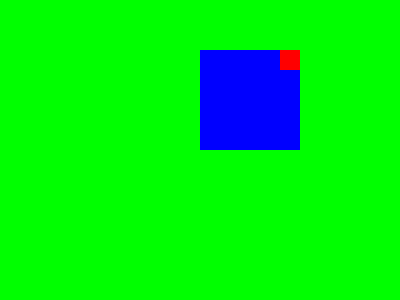
\includegraphics[width=0.5\textwidth]{images/ch18-spritebatch-rotation-easygl.png}
\end{figurealt}
\caption{Output of the rotate-around-origin \cnaclass{SpriteBatch} scene from
Figure~\ref{fig:ch17-spritebatch-rotation}, rendered by \texttt{EasyGL} through OpenGL ES under
\texttt{Xvfb}. The retained EasyGL and SDL Renderer images are pixel-identical for this fixture;
the comparison does not extend beyond the recorded scene.}
\label{fig:ch18-spritebatch-rotation}
\end{figure}

The two retained $400\times300$ PNG files are byte-for-byte identical. This establishes
cross-renderer agreement for the named fixture only; the D3D9 oracle corpus elsewhere in this
chapter covers a broader set of scenes.

\section{OPENGL4: modern core without the EasyGL family}

\texttt{OPENGL4} is an independent implementation built against system OpenGL and a
hand-rolled function loader.  It targets GLSL~410 core.  Neither its source tree nor its
shader path is shared with EasyGL, so \texttt{OPENGL33} and \texttt{OPENGL4} are not two
settings on one renderer despite their adjacent version numbers.

The distinction is useful in both directions.  EasyGL carries profile rewriting and Web/ES
compatibility workarounds; \texttt{OPENGL4} can assume a modern desktop core surface.  A bug
in one shader generator or context path is therefore not evidence about the other.

The renderer owns real 2D targets, MRT, and occlusion-query paths.  Its extended primitive
dispatch is nevertheless hybrid: \texttt{BindProgramForStride()} selects a native program
for supported vertex/effect combinations, while an unmatched combination reaches the colored
draw tail.  That tail is a bounded internal fallback, not the base-class inheritance defect,
but it can still discard effect intent.  Tests of custom layouts must therefore verify pixels
or bindings, not merely that a draw call returned.

\begin{sourcenote}
For selection and bug triage, treat \texttt{OPENGL33} as an EasyGL profile and
\texttt{OPENGL4} as a separate renderer family.  The public names encode neither shared code
nor an automatic upgrade path.
\end{sourcenote}

\section{PORTABLEGL: OpenGL-shaped software, not a GPU driver}

\texttt{PORTABLEGL} occupies a different point on the portability axis.  CNA fetches a pinned
PortableGL revision and executes the pipeline on the CPU.  Its shaders are C function
pointers, not GLSL, and it creates no GPU resource of any kind.

That makes it valuable for deterministic experiments and systems without a graphics device,
but its boundaries are explicit:

\begin{itemize}
  \item its extended primitive paths are native to the CPU pipeline;
  \item \cnaclass{RenderTarget2D}, MRT, and occlusion queries are not supported;
  \item unsupported GPU features should be treated as deliberate refusals rather than as
        promises that happen to run slowly in software.
\end{itemize}

PortableGL is consequently not a substitute for EasyGL conformance evidence.  Agreement
between their pixels can be useful, but it compares two independent implementations with
different rasterization and shader machinery.

\section{A ten-identity decision map}

The complete OpenGL-named surface now separates cleanly:

\begin{longtable}{p{0.24\textwidth}p{0.30\textwidth}p{0.31\textwidth}}
\toprule
Need & Candidate & Principal caution \\
\midrule
\endfirsthead
\toprule
Need & Candidate & Principal caution \\
\midrule
\endhead
desktop fixed function & \texttt{OPENGL1} & optional FBO/query surface \\
GLSL~1.10 compatibility & \texttt{OPENGL2} & legacy language and context \\
ES~1.1 fixed function & \texttt{OPENGLES1} & specialized system dependency \\
ES~2/WebGL~1 & \texttt{OPENGLES2}, \texttt{WEBGL1} & narrow profile ceilings \\
ES~3/WebGL~2 & \texttt{OPENGLES3}, \texttt{WEBGL2} & the two names share the same internal profile path \\
desktop EasyGL & \texttt{OPENGL33} & EasyGL family, not \texttt{OPENGL4} \\
desktop core GL & \texttt{OPENGL4} & hybrid tail for unmatched draw combinations \\
CPU OpenGL-shaped execution & \texttt{PORTABLEGL} & no GPU targets, MRT, or queries \\
\bottomrule
\end{longtable}

Across all ten identities, the selector name is only the beginning of the contract.  Record
the implementation family, shader language, context source, optional-function boundary, and
verification environment alongside it.  Those five facts explain more real portability
failures than the nominal GL version alone.
